%----------------------------------------------------------------------------------------
% PACKAGES AND DOCUMENT CONFIGURATIONS
%----------------------------------------------------------------------------------------

  \documentclass[12pt]{article}

  \usepackage{hyperref}
  \usepackage{fancyhdr} % Required for custom headers
  \usepackage{lastpage} % Required to determine the last page for the footer
  \usepackage{extramarks} % Required for headers and footers
  \usepackage[usenames,dvipsnames]{color} % Required for custom colors
  \usepackage{graphicx} % Required to insert images
  \usepackage{listings} % Required for insertion of code
  \usepackage{courier} % Required for the courier font
  \usepackage{lipsum} % Used for inserting dummy 'Lorem ipsum' text into the template
  \usepackage{wrapfig}
  \usepackage{color}
  \usepackage{lscape}
  \usepackage{pbox}

 \graphicspath{ {../Figures/} }% figures are taken from this folder
 \setlength{\intextsep}{3ex} % set space above and below in-line float (figures, tables etc)
\setlength{\floatsep}{2ex} % space between floats
%\setlength{\abovecaptionskip}{1ex} % space above float caption
%\setlength{\belowcaptionskip}{5ex} % space below float caption

% numerotation for figures and tables
\renewcommand{\thefigure}{\arabic{section}.\arabic{figure}}
\renewcommand{\thetable}{\arabic{section}.\arabic{table}}


  \setlength\parindent{0pt} % Removes all indentation from paragraphs
  \renewcommand{\labelenumi}{\alph{enumi}.} % Make numbering in the itemize environment by letter rather than number (e.g. section 6)

  % Margins
  \topmargin=-0.4in
  \evensidemargin=0.2in
  \oddsidemargin=-0.2in
  \textwidth=7.0in
  \textheight=9.0in
  % \headsep=0.25in

  % \linespread{1.1} % Line spacing

  \definecolor{dkgreen}{rgb}{0,0.6,0}
  \definecolor{gray}{rgb}{0.5,0.5,0.5}
  \definecolor{mauve}{rgb}{0.58,0,0.82}
  \definecolor{greyish}{rgb}{0.96,0.96,0.96}

  \lstset{
    backgroundcolor=\color{greyish},   % choose the background color; you must add \usepackage{color} or \usepackage{xcolor}
    frame=tblr,
    numbers=left,                       % where to put the line-numbers; possible values are (none, left, right)
    numbersep=5pt,                   % how far the line-numbers are from the code
    numberstyle=\tiny\color{mygray}, % the style that is used for the line-numbers
    language=Ruby,
    aboveskip=3mm,
    belowskip=3mm,
    showstringspaces=false,
    columns=flexible,
    basicstyle={\footnotesize\ttfamily},
    numbers=none,
    numberstyle=\tiny\color{gray},
    keywordstyle=\color{blue},
    commentstyle=\color{dkgreen},
    stringstyle=\color{mauve},
    breaklines=true,
    breakatwhitespace=true
    tabsize=1
  }

  \begin{document}
  \begin{titlepage}

%----------------------------------------------------------------------------------------
% TITLE PAGE INFORMATION
%----------------------------------------------------------------------------------------
 \newcommand{\HRule}{\rule{\linewidth}{0.5mm}} % Defines a new command for the horizontal lines, change thickness here
  \begin{center} % Center everything on the page

  %----------------------------------------------------------------------------------------
  % HEADING SECTIONS
  %----------------------------------------------------------------------------------------
  \textsc{\large Faculty of Computers, Informatics and Microelectronics}\\[0.5cm]
  \textsc{\large Technical University of Moldova}\\[1.2cm] % Name of your university/college
  \vspace{35 mm}
  \textsc{\Large APA}\\[0.5cm] % Major heading such as course name
  %\textsc{\large Laboratory work \#1-3}\\[0.5cm] % Minor heading such as course title
  \textsc{\large Laboratory work \# 1}\\[0.5cm] % Minor heading such as course title

  %----------------------------------------------------------------------------------------
  % TITLE SECTION
  %----------------------------------------------------------------------------------------
  \vspace{10 mm}
  \HRule \\[0.4cm]
  { \LARGE \bfseries Name of the 1st Laboratory Work }\\[0.4cm] % Title of your document
  \HRule \\[1.5cm]

  %----------------------------------------------------------------------------------------
  % AUTHOR SECTION
  %----------------------------------------------------------------------------------------
      \vspace{30mm}

      \begin{minipage}{0.4\textwidth}
      \begin{flushleft} \large
      \emph{Authors:}\\
      Your \textsc{Name}
      \end{flushleft}
      \end{minipage}
      ~
      \begin{minipage}{0.4\textwidth}
      \begin{flushright} \large
      \emph{Supervisor:} \\
      Irina \textsc{Cojanu} % Supervisor's Name
      \end{flushright}
      \end{minipage}\\[4cm]

      \vspace{5 mm}
      % If you don't want a supervisor, uncomment the two lines below and remove the section above
      %\Large \emph{Author:}\\
      %John \textsc{Smith}\\[3cm] % Your name

      %----------------------------------------------------------------------------------------
      % DATE SECTION
      %----------------------------------------------------------------------------------------

      {\large \today}\\[3cm] % Date, change the \today to a set date if you want to be precise

      %----------------------------------------------------------------------------------------
      % LOGO SECTION
      %----------------------------------------------------------------------------------------

      %\includegraphics{Logo}\\[1cm] % Include a department/university logo - this will require the graphicx package

      %----------------------------------------------------------------------------------------

      \vfill % Fill the rest of the page with whitespace
      \end{center}
      \end{titlepage}

      % \newpage
      % \tableofcontents
      % \newpage

%----------------------------------------------------------------------------------------
% Introduction
%----------------------------------------------------------------------------------------

  \section{Introduction}

  \subsection{Topic}

  The name of the laboratory work

  \subsection{Task}

  \begin{itemize}
    \renewcommand{\labelitemi}{$\circ$}
    \item 1st task
    \item 2nd task
    \item 3rd task
  \end{itemize}

%----------------------------------------------------------------------------------------
% Implementation
%----------------------------------------------------------------------------------------

  \section{Implementation}

  \subsection{Questions}

  \begin{itemize}
    \renewcommand{\labelitemi}{$\circ$}
    \item Q1
    \item Q2
    % \item
   \end{itemize}


    \subsection{Conclusion/Results}

 \subsection{Examples of formulas}
Below is a text with some formulas. You should specify each variable being used, unless this variable was not mentioned in a formula mentioned befiore.

Consider a symmetric profile of a hydrodynamic blade in a fluid flow with uniform velocity $\overrightarrow{V}_{\infty
} $. In the fixing point of the symmetric blade with the boom $OO^{\prime }$
we consider two coordinate systems, namely: the $O^{\prime }xy$\ system with
axis $O^{\prime }y$\ oriented in the direction of velocity vector $\overrightarrow{V}_{\infty }$, and axis $O^{\prime }x$\ normal to this direction; and the $O^{\prime }x^{\prime }y^{\prime }$\ system with axis $O^{\prime }y^{\prime }$\ oriented along the boom direction $OO^{\prime }$, and axis $O^{\prime }x^{\prime }$ normal to this direction. Points $A$\ and $B$\ correspond to the trailing edge and the leading edge, respectively. The angle of attack $\alpha $\ is the angle between the profile chord $AB$\ and $\overrightarrow{V}_{\infty}$, and the positioning angle $\varphi $\ is the
angle between the boom $OO^{\prime }$\ and $\overrightarrow{V}_{\infty }$.

The hydrodynamic force $\overrightarrow{F}$\ has its lift and drag components in directions $O^{\prime }x$\ and $O^{\prime }y$, respectively, given by:
\begin{eqnarray}
F_{L} &=&\frac{1}{2}C_{L}\rho _{\infty }V_{\infty }^{2}S_{p},  \label{1.1} \\
F_{D} &=&\frac{1}{2}C_{D}\rho _{\infty }V_{\infty }^{2}S_{p},  \label{1.2}
\end{eqnarray}
where $\rho $\ is the fluid density, $V_{\infty }$\ is the flow velocity, $S_{p}=ch$ ($c$ is the chord length, $h$ is the blade height) represents the lateral surface area of the blade, and $C_{L}$\ and $C_{D}$\ are the
dimensionless hydrodynamic coefficients, lift and drag coefficients, respectively. Coefficients $C_{L}$ and $C_{D}$ are dependent on the angle of attack $\alpha $, the Reynolds number $Re$ and the hydrodynamic shape of the blade profile. The components of the hydrodynamic force in the coordinate system $O^{\prime }x^{\prime }y^{\prime }$ are given by
\begin{eqnarray}
F_{x^{\prime }} &=&-F_{L}\sin \varphi +F_{D}\cos \varphi,  \label{1.3} \\
F_{y^{\prime }} &=&F_{L}\cos \varphi +F_{D}\sin \varphi , \label{1.4}
\end{eqnarray}
where $F_L$ and $F_D$ are determined form relations (\ref{1.1}) and (\ref{1.2}). 

The torque at the rotor axis $O$ developed by the blade $i$ is
\begin{equation}
T_{r,i}=F_{x^{\prime }}\cdot \left\vert OO^{\prime }\right\vert  \label{1.5}
\end{equation}%
and the total torque developed by all blades
\begin{equation}
T_{r\Sigma }=\sum\limits_{i=1}^{N_{b}}T_{r,i},  \label{1.6}
\end{equation}%
where $N_{b}$ is the number of the rotor's blades.

Since the hydrodynamic force with components (\ref{1.3}--\ref{1.4}) does not have its application point in the
origin of the blade axis system $O^{\prime }$, it will produce a pitching
moment with respect to a reference point chosen to be located at $\frac{1}{4}$ of the chord distance from the leading edge. The pitching moment, is computed by
\begin{equation}
M=\frac{1}{2}C_{M}\rho _{\infty }V_{\infty }^{2}cS_{p}  \label{1.7}
\end{equation}
where $C_{M}$ represents the pitching moment hydrodynamic coefficient.

\subsection{Examples of tables}

You might use a large variety of styles for tables. Don't forget to refer to the tables in the text and comment them.

\begin{table}[h!]
\centering
\caption{Estimation for computational effort associated to RANS and LES methods}
{
\renewcommand{\arraystretch}{2}
\begin{tabular}{ c|c|c|c|c }
\hline           
 Method & \pbox{4cm}{Cells} &\pbox{5cm}{Timesteps} &  \pbox{7cm}{No. of internal ops \\ per timestep} & \pbox{7cm}{Relativ effort \\ compared with RANS} \\ \hline \hline
 RANS & $\approx 10^6$ & $\approx 10^2-10^3$ & $1$ & $1$ \\ 
 LES & $\approx 10^9$ & $\approx 10^5$ & $1-10$ & $\approx 10^5-10^6$ \\ \hline 
\end{tabular}
}
\label{LesRans}
\end{table}

\begin{table}[ht!]
\centering
\caption{Discretisation parameters for windrose wheel surface}
{
\renewcommand{\arraystretch}{1.25}
\begin{tabular}{ c|c|c|c }
\hline           
       & Element Size & Curvature Normal  Angle & Growth Rate \\ \hline \hline
 Hub & $9$ mm & $10^o$ & 1,17 \\ 
 Root & $4,5$ mm & $4^o$ & 1,17 \\ 
 TLE & $0,7$ mm & $1^o$ & 1,135 \\
 Tips & $0,4$ mm & $1^o$ & 1,135 \\ 
 Blades & $8,5$ mm & $5^o$ & 1,165 \\ \hline 
\end{tabular}
}
\label{Tab3_1}
\end{table}

\subsection{Examples of listings}The listings of the code can be inserted using the package listings and setting up your own style, that will enhance greatly the readability of your code. The style for listing is defined in the thesis style fyle. For more details check \url{http://en.wikibooks.org/wiki/LaTeX/Source_Code_Listings} or listings package documentation. Below there are presented two examples. In listing \ref{list1} the code is taken directly from the file, while in the second example the code is inserted directly in the text, see listing \ref{list2}.  

\lstinputlisting[language=Java, caption={Java example, code is included from a fyle}, label=list1]{../SrcCode/ViewFacade.java}


% \begin{lstlisting}[language=Python, caption={Python example, code is listed}, label=list2]
% import numpy as np
 
% def incmatrix(genl1,genl2):
%     m = len(genl1)
%     n = len(genl2)
%     M = None #to become the incidence matrix
%     VT = np.zeros((n*m,1), int)  #dummy variable
 
%     #compute the bitwise xor matrix
%     M1 = bitxormatrix(genl1)
%     M2 = np.triu(bitxormatrix(genl2),1) 
 
%     for i in range(m-1):
%         for j in range(i+1, m):
%             [r,c] = np.where(M2 == M1[i,j])
%             for k in range(len(r)):
%                 VT[(i)*n + r[k]] = 1;
%                 VT[(i)*n + c[k]] = 1;
%                 VT[(j)*n + r[k]] = 1;
%                 VT[(j)*n + c[k]] = 1;
 
%                 if M is None:
%                     M = np.copy(VT)
%                 else:
%                     M = np.concatenate((M, VT), 1)
 
%                 VT = np.zeros((n*m,1), int)
 
%     return M
% \end{lstlisting}

\newpage
\subsection{Examples of images}

\begin{figure}[!ht]
\renewcommand\thefigure{I.1} % Make this Figure I.1
\centering
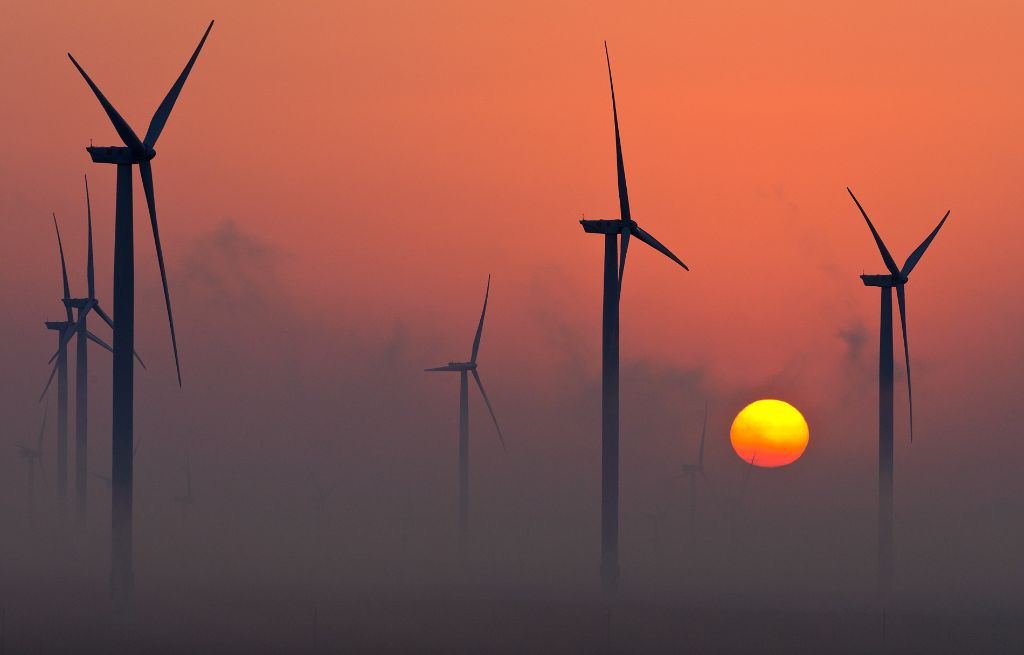
\includegraphics[width=10cm]{1-WindF-2}
\caption{Evolution of the aerodynamic tunnel simulations versus the CFD simulations}\label{figI1}
\end{figure}

   % Example of how to add an image
    \begin{minipage}[b]{1.0\linewidth}
      \begin{center}
        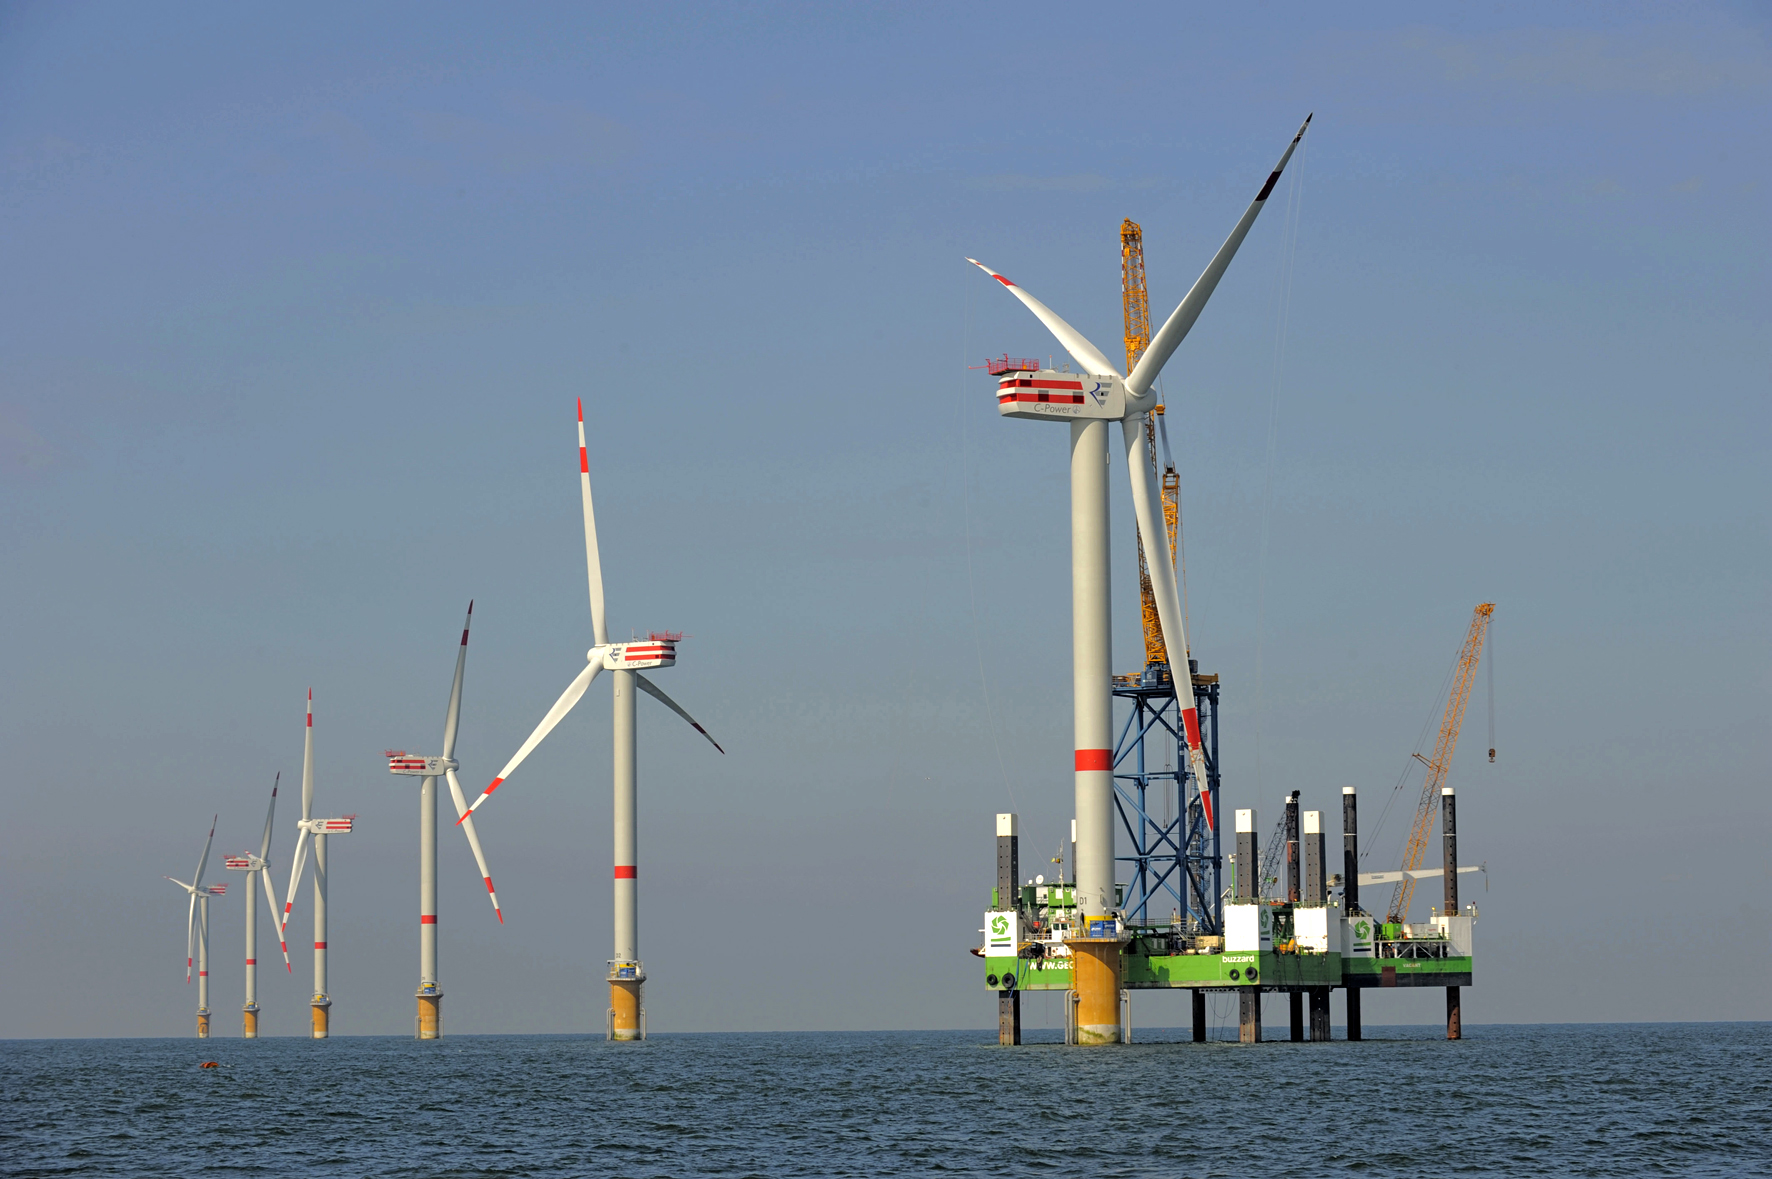
\includegraphics[width=0.9\textwidth]{1-WindF-1}
         \\ Fig. 1 Name of the figure 1
      \end{center}
    \end{minipage}

  
\end{document}